\section{Diverse}\label{Diverse}
Dette afsnit dækker over klasserne der ikke ligger under en bred kategori af klasser.

\subsection{Project}
\texttt{Project} klassens formål er at holde på informationen om elementerne i vejnettet. Derudover holder \texttt{Project} klassen også på brugerens indstillinger for simuleringerne der udføres. Disse indstillinger er gemt i en instans af klassen \texttt{SimulationSettings}. Når \texttt{Project} klassen instansieres, tilføjer constructoren en \texttt{Default} type til \texttt{RoadTypes}, \texttt{VehicleTypes} og \texttt{DestinationTypes}, hvilket er listerne der gemme på alle typerne af deres slags. \texttt{Default} værdierne kan ikke slettes, da det ikke vil give mening for simuleringen at veje, køretøj og destinationer eksisterede uden en type, og programmet ville blive termineret. 

\begin{figure}[H]
\begin{lstlisting} 
public object Clone()
{
  MemoryStream memory = new MemoryStream();
  BinaryFormatter formatter = new BinaryFormatter();
  formatter.Serialize(memory, this);
  memory.Position = 0;
  return formatter.Deserialize(memory);
}
\end{lstlisting}
\caption{Project.cs}\label{Project}
\end{figure}

\texttt{Project} klassen implementerer interfacet \texttt{ICloneable}, der beder om en implementation af \texttt{Clone()}, der returnerer en kopi af en instans af et \texttt{Project}. Implementationen af \texttt{Clone()} funktionaliteten er vist på figur \ref{Project}, hvor instansen af \texttt{Project} bliver seraliseret vha. \texttt{BinaryFormatter} klassen, og derefter deserliseret samt returneret. Grunden til \texttt{Clone()} funktionen er at lave en 'deep copy' af projektet, da Simulation klassen har brug for en identisk men adskildt kopi, så køretøjerne i \texttt{Primary} og \texttt{Secondary} simuleringerne ikke kan se og holde for hinanden. En \texttt{MemberwiseClone()} som alle objekter har adgang til, laver kun en 'shallow copy', hvilket vil sige at noderne og vejene stadig ville være referencer til de samme som i det første \texttt{Project}.

\subsection{SimulationSettings}
\begin{figure}[H]
\begin{lstlisting} 
// Defaults
public SimulationSettings()
{
  StepSize = 100;
  VehicleSpace = 2;
  IncommingRange = 10;
  PrimaryCarCount = 1000;
  PrimaryInbound = 100;
  PrimaryOutbound = 100;
  PrimaryToDestTime = 28800000; // 08:00
  PrimaryToHomeTime = 57600000; // 16:00
  PrimaryTimeSpread = 14400000; // 4h
  SecondaryCarCount = 1000;
  SecondaryInbound = 100;
  SecondaryOutbound = 100;
  SecondaryToDestTime = 28800000; // 08:00
  SecondaryToHomeTime = 57600000; // 16:00
  SecondaryTimeSpread = 14400000; // 4h
}
\end{lstlisting}
\caption{SimulationSettings}\label{SimulationSettings}
\end{figure}

\texttt{SimulationSettings}, som kan ses på figur \ref{SimulationSettings}, indeholder alle indstillingerne der bliver brugt i en simulering. Constructoren til klassen sætter variablerne til de definerede værdier. Værdierne kan justeres gennem brugerfladen \texttt{GUIMenuSettingsSimulation}. I brugerfladen kan værdierne tilgås gennem nogle \texttt{NumericUpDown} elementer, hvor minimum og maximum er sat for at kontrollerer hvordan simuleringen kan indstilles. På tabel \ref{SimulationLimits} kan begrænsningerne ses. Yderligere er der også regler brugeren skal overholde når indstillingerne skal sættes. \texttt{Inbound} og \texttt{Outbound} skal være lavere end \texttt{VehicleCount}, og \texttt{TimeSpread} må ikke gøre det muligt at køretøjer kan starte deres rejser uden for tidsrummet mellem 0 og 86400000 millisekunder. Der er lavet en brugerflade, der kan tilgås ved at trykke på en \texttt{Info} knap, som beskriver hvad variablerne betyder, da navnene muligvis kunne blive misforstået.

\begin{table}[]
\centering
%\begin{adjustbox}{height=0.12\textheight}
\begin{tabular}{| c | c | c |}
  \hline
Variable & Minimum & Maximum \\
  \hline
StepSize & 10 & 100 \\
  \hline
VehicleSpace & 0 & 100 \\
  \hline
IncomingRange & 0 & 100 \\
  \hline
CarCount & 0 & 10000 \\
  \hline
Inbound & 0 & 10000 \\
  \hline
Outbound & 0 & 10000 \\
  \hline
ToDestTime & 0 & 86400000 \\
  \hline
ToHomeTime & 0 & 86400000 \\
  \hline
TimeSpread & 0 & 86400000 \\
  \hline
\end{tabular}
%\end{adjustbox}
\caption{Begrænsninger for simulering indstillingerne}\label{SimulationLimits}
\end{table}

\subsection{Data}
\texttt{SimulationData} er en klasse der indeholder dataen fra køretøjerne (\texttt{VehicleData}) fra en \texttt{Primary} og \texttt{Secondary} simulering, og en kopi af projektet simuleringen blev kørt på. Det er denne klasse der bliver gemt i en fil efter simuleringen, så brugeren kan åbne den senere gennem \texttt{SimulationView} brugerfladen. \texttt{VehicleData} indeholder arrays af punkterne der blev optaget gennem simuleringen, tiden på starten af rejsen mod og fra destinationen, samt køretøjets type. Ved begge klasser sættes dataen ind gennem constructoren, og det kan derefter ikke ændres igen, da egenskaberne for variablerne er med private settere. Data klasserne kan ses på figur \ref{SimData} og \ref{VehicleData}.

\begin{figure}[H]
\centering
\begin{minipage}{0.45\textwidth}
\centering
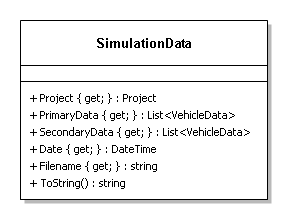
\includegraphics[width=1\textwidth,height=\textheight,keepaspectratio]{Pictures/Klassediagram/SimulationData}
\caption{SimulationData klassen}
\label{SimData}
\end{minipage}\hfill
\begin{minipage}{0.45\textwidth}
\centering
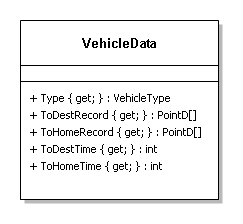
\includegraphics[width=1\textwidth,height=\textheight,keepaspectratio]{Pictures/Klassediagram/VehicleData}
\caption{VehicleData klassen}
\label{VehicleData}
\end{minipage}
\end{figure}

\subsection{MathExtension}
\texttt{MathExtension} er en klasse der er lavet for at håndtere udregningerne fra \texttt{Point} til \texttt{Point}, fra \texttt{PointD} til \texttt{PointD} samt en kort kovertering af km/h til m/ms. Der gøres bruge af klasser fra \texttt{Math} bibliotek. Måden vi udregner km/h til m/ms, er ved at tage km/h og dividere med 3600(60*60), se udregning \ref{ConvertKmhToMms}. Vi benytter os af afstandsformlen i \texttt{MathExtension}, hvor vi beregner afstanden mellem to noder via deres koordinater \ref{AfstandsFormel}. Afstandsformlen benyttes flere steder i programmet, men primært i \texttt{Pathfinder} og \texttt{Vehicle}, og konverteringen til meter på millisekund bliver kun bruger i \texttt{Vehicle.Drive()}.

\begin{equation} \label{ConvertKmhToMms}
km/h / 3600
\end{equation}

\begin{equation} \label{AfstandsFormel}
\sqrt{(x_2 - x_1)^2 + (y_2 - y_1)^2}
\end{equation}

\subsection{Vector2D}
\begin{figure}[H]
\begin{lstlisting}
public void Scale(double scalar)
{
  X *= scalar;
  Y *= scalar;
}
public void ToUnit()
{
  double magnitude = Length;
  X /= magnitude;
  Y /= magnitude;
}
public static Vector2D FromRoad(Road road)
{
  Vector2D vector = new Vector2D();
  vector.X = road.To.Position.X - road.From.Position.X;
  vector.Y = road.To.Position.Y - road.From.Position.Y;
  return vector;
}
\end{lstlisting}
\caption{Vector2D klasse}\label{Vector2D}
\end{figure}

Formålet med \texttt{Vector2D} klassen er at gøre det nemt at flytte køretøjer, som bliver gjort i \texttt{TranslateVehicle()} metoden, der ligger i \texttt{Vehicle} klassen. \texttt{Vector2D} klassen har tre metoder, \texttt{Scale()}, \texttt{ToUnit()} og \texttt{FromRoad()}, som vises på figur \ref{Vector2D}. Den første metode \texttt{Scale()} ganger vektoren op med en scalar der bliver taget som input parameter. I \texttt{ToUnit()} bliver vektorens \texttt{X} og \texttt{Y} divideret med størrelsen af vektoren, således at vektorens størrelse bliver lig 1. \texttt{FromRoad()} metoden laver en \texttt{Vector2D} ud fra en \texttt{Road} instans koordinater.

